\section{Results}

At the conclusion of Run 3, in December of 2013, a total of 10 Bq of tritium was injected into LUX and removed. A total 300,000 events were observed in the 251 kg active volume of LUX, of which 170,000 events were in the 145 kg fiducial volume at the nominal LUX electric field of 180~V/cm. Another 4,500 fiducial events were collected in a special run at a reduced field of 105~V/cm. We correct the S1 and S2 signals for spatial and temporal effects such as the light collection efficiency and the free electron lifetime with $ ^{83m}$Kr data as described in \cite{lux-reanalysis}. 


\fixit{Data for analysis is selected using cuts identical to the WIMP search analysis. Within an event window single scatters are selected by pairing an S1 with a single S2.  The S1 is measured using spike counting in the PMTs, requiring a minimum two fold coincidence from PMTs that are not in neighboring channels. The S2 signal is required to be greater than 150 phd (6 extracted electrons) to ensure accurate position reconstruction. The events are further required to be within a fiducial volume of 6 to 46 cm drift and less than 20 cm radius.}

We interpret the data in terms of the combined energy model for electron recoils \cite{Platzman}, where the total energy of an event is directly proportional to the number of quanta produced (ionization electrons plus scintillation photons):

\begin{equation}
E_{total} = W \cdot (n_{\gamma} + n_e ),
\label{platzman_eq}
\end{equation}

\noindent
where $E_{total}$ is the energy of the deposition in keV and  $n_\gamma$ and $n_e$ are the number of photons and electrons respectively. We employ the combined energy model because it reproduces well the true energy of the event, while the individual photon and electron signals are non-linear in energy due to the effects of recombination. We use a $W$-value of 13.7 $\pm$ 0.2 eV/quanta \cite{Dahl_Thesis}. In LUX $n_{\gamma}$ and $n_e$ are proportional to the S1 and S2 signals, with gain factors $g_1$ and $g_2$: 
%We use a $W$ value of 13.7 $\pm$ 0.2 eV/quanta \cite{Dahl_Thesis}. In LUX $n_{\gamma}$ and $n_e$ are proportional to the S1 and S2 signals, with gain factors $g_1$ and $g_2$:

\begin{equation}
E_{total} = W \cdot \left(\frac{S1}{g_1} + \frac{S2}{g_2} \right),
\label{energy_eq}
\end{equation}

\noindent
\fixit{where S1 and S2 have units of photons detected (phd) and $g_1$ and $g_2$ have units of phd per quantum. $g_1$ is the average light collection efficiency times the average quantum efficiency of the PMT arrays, while $g_2$ is the product of the electron extraction efficiency at the liquid-gas surface and the average single electron size in phd. $g_1$ and $g_2$ are measured with line source data and single electron events in LUX Run 3 to be $0.117 \pm 0.003$ phd/photon and $12.05 \pm 0.8$ phd/electron\cite{lux-reanalysis, lux-prd}. For the December 2013 tritium calibration presented here, the gains g1 and g2 are slightly shifted as measured from $\rm ^{83m}Kr$ calibration data, $g_1$ and $g_2$ are measured to be $0.114 \pm 0.003$ phd/photon and $12.0 \pm 0.8$.}

%are constrained by optimizing the combined energy model to the true tritium spectral shape \cite{Tritium_Eq_Simpson} convolved with detector resolution. We find values of $g_1$ = \gone  phd/photon ~and  $g_2$ = \gtwo phd/electron.  The difference between these values with those quoted in Ref. \cite{lux-reanalysis, lux-prd} is taken as a systematic error for the results present in Ref. \cite{lux-reanalysis, lux-prd}.

\begin{figure}[h!]
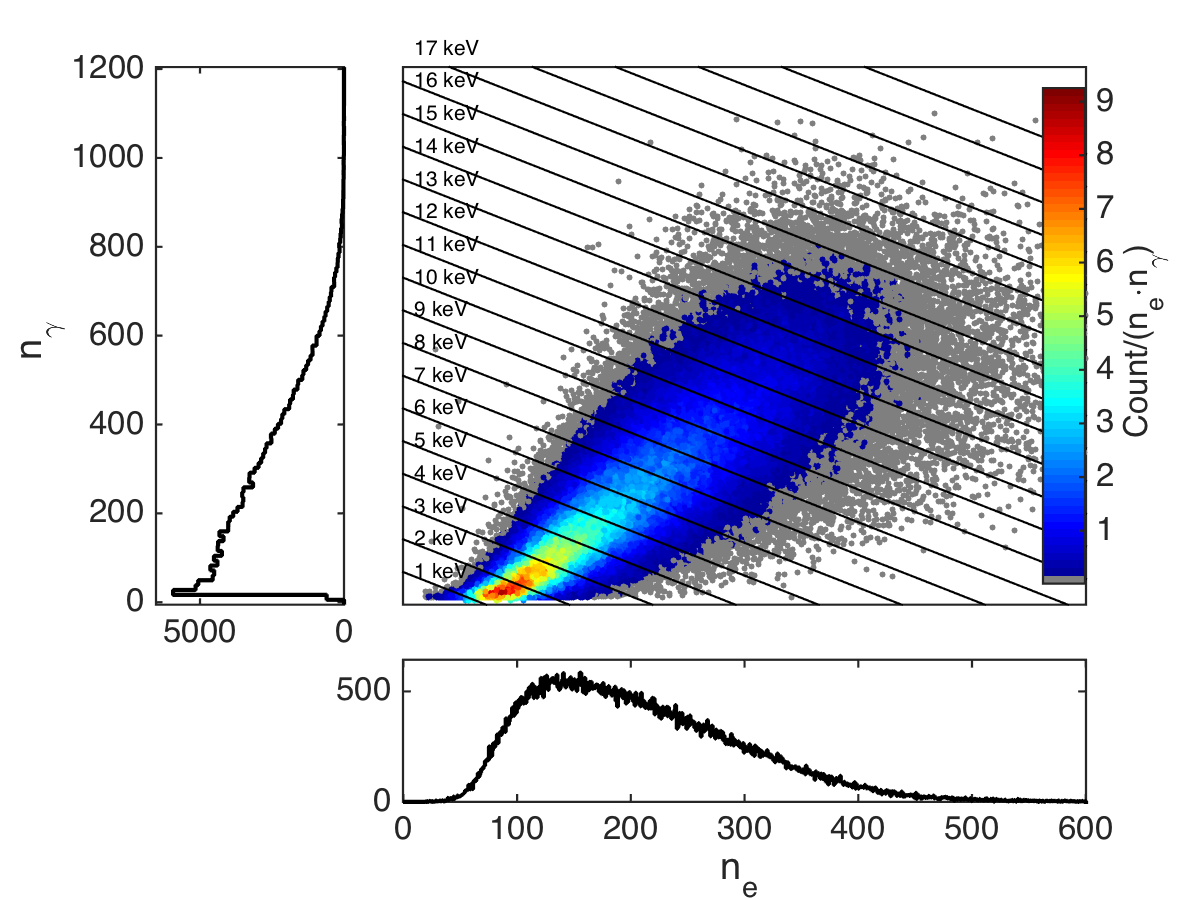
\includegraphics[width=90mm]{fig/tritium_scatter.png}
\caption{Scatter plot of $n_e$ vs $n_{\gamma}$ for 170,000 fiducial tritium events at 180~V/cm. Lines of constant energy are indicated assuming a $W$-value of 13.7~eV. The data is projected into $n_e$ and $n_{\gamma}$ histograms on each axis.}
\label{fig:tritium-scatter}
\end{figure}


\begin{figure}[h!]
\begin{center}
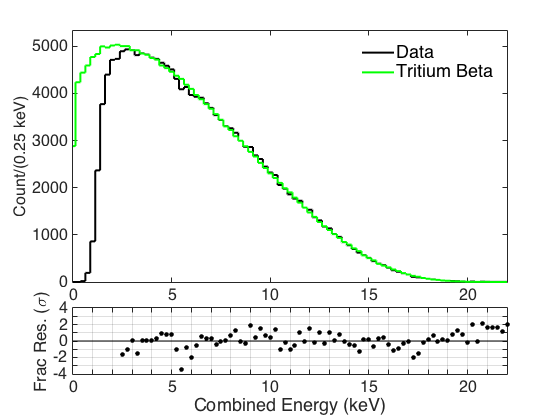
\includegraphics[width=90mm]{fig/tritium-spectrum-linear.png}
\caption{The tritium energy spectrum measured by LUX with the combined energy model (black) compared to two models: a pure tritium spectrum (dashed blue), and a tritium spectrum convolved with detector resolution  ($\frac{\sigma_E}{W} = \sqrt{\sigma^2(n_{\gamma})+ \sigma^2(n_e)}$.) \fixit{The fractional residuals between the data and the simulated spectrum correspond to a $\chi^2_{red}$=1.35}}
\label{fig:tritium-spectrum}
\end{center}
\end{figure}

%S1 ($ \sigma(n_{\gamma}))$ and S2 ($\sigma(n_e)$)

A scatter plot of $n_e$ vs $n_{\gamma}$ for the tritium data at 180~V/cm is shown in Fig. \ref{fig:tritium-scatter}, along with the projected histograms on each axis. Contours of constant energy in 1~keV intervals are also plotted, derived from Eq. \ref{platzman_eq}. 


The tritium energy spectrum, obtained by projecting the data along the lines of constant energy, is shown in Fig. \ref{fig:tritium-spectrum}. The data are compared to an ideal tritium spectrum \cite{Tritium_Eq_Simpson}, with no detector effects, and a tritium spectrum with an energy smearing factor of $ \frac{\sigma_E}{W} = \sqrt{\sigma(n_{\gamma})^2 + \sigma(n_e)^2}$, where $ \sigma(n_{\gamma})$ and $ \sigma(n_e)$ represent the detector resolution for photon and electron counting. In the fit the models are normalized to the data. The ratio of the data to the smeared theoretical spectrum is shown in Fig. \ref{fig:ER-threshold}, along with an empirical fit to an error function. The effective 50\% energy threshold for ER events is found to be 1.30 $\pm$ 0.013~keV. The excellent agreement between data and theory from 3~keV to the endpoint of the tritium spectrum supports the combined energy model in Eq.~\ref{platzman_eq}.

\begin{figure}[h!]
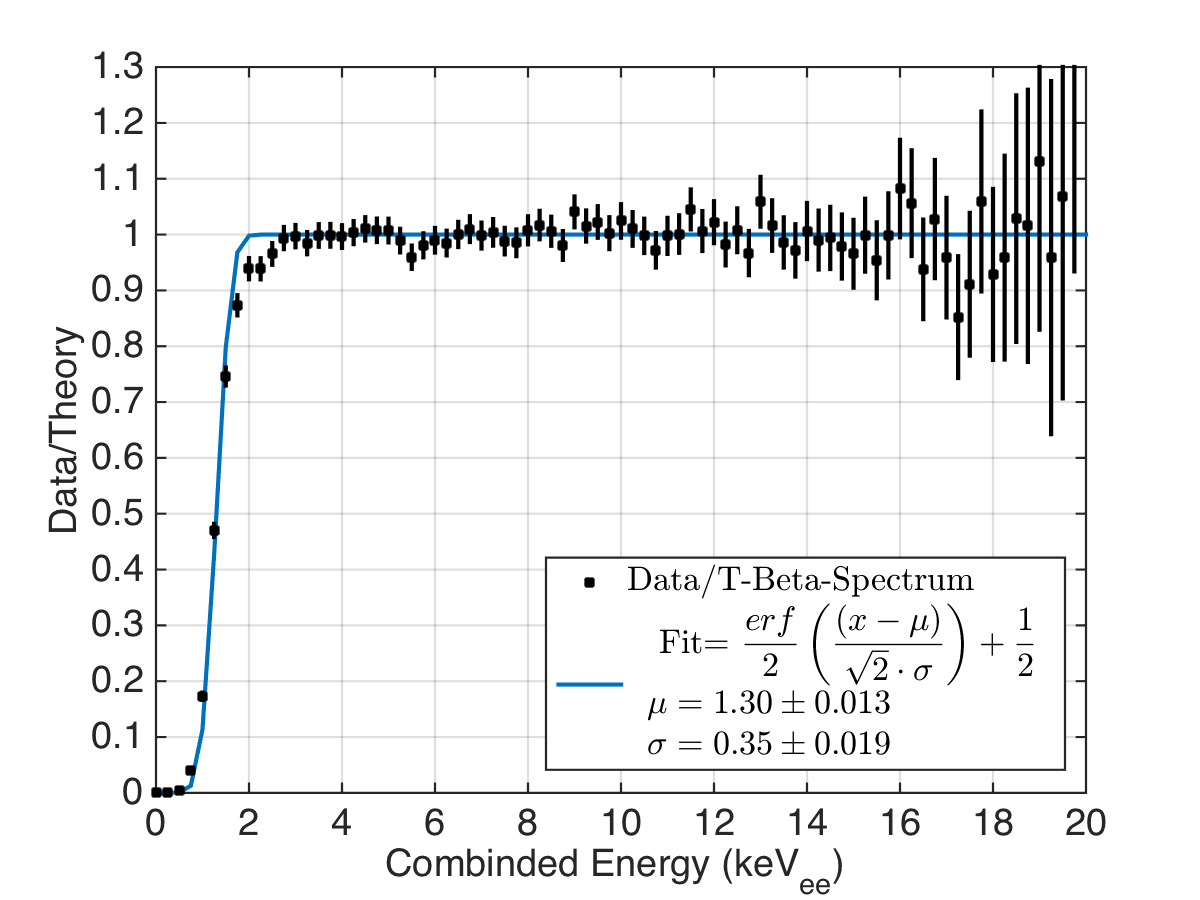
\includegraphics[width=90mm]{fig/E_Thres_Fit.png}
\caption{Ratio of the measured tritium energy spectrum and the true one convolved with the detector resolution. A fit to an error function is shown.}
\label{fig:ER-threshold}
\end{figure}


%Individual events on the plot are smeared by detector resolution and electron-ion pair recombination fluctuations. Detector resolution is comprised of statistical fluctuations in counting photons and electrons in the S1 and S2 channel. The finite resolution in S1 and S2 smear events along the vertical and horizontal axis, respectively. Recombination fluctuations ($ \sigma(R)$) smear events along the contours of constant energy, and thus cancel out in the combined energy model of Eq.\ref{platzman_eq}. 


The mean light and charge yields of ER events in LUX are obtained by dividing the mean light and charge signals by the combined energy in each energy bin. The result is shown for 180~V/cm and 105~V/cm in Fig. \ref{fig:ER-LY-QY} along with NEST v0.98 model predictions at each field \cite{NEST_2013}. For these plots a small correction has been applied to the data to account for smearing of tritium events across energy bins due to the energy resolution and the spectral shape \cite{Dobi_Thesis}\footnote{We have verified with an internal $\rm ^{83m}Kr$ calibration source that the light yield of LXe is unaffected by the presence of CH$_4$ at concentrations up to $\sim$1 part per million. For the CH$_3$T measurements reported here the concentration was ($<$ $10\times10^{-12}$ g/g). }.  NEST v0.98 describes the data approximately, but predicts too much light yield and too little charge yield above 6~keV. Note that NEST v0.98 lacks direct input measurements in this energy range and electric field, so a modest disagreement is not unexpected. A more recent version of NEST (v1.0) has been tuned to reproduce the LUX tritium data shown here faithfully. The yields from tritium at 180 and 105 V/cm plotted can be found in Table \ref{table:Yields} and Table \ref{table:Yields_100}.

\begin{figure}[h!]
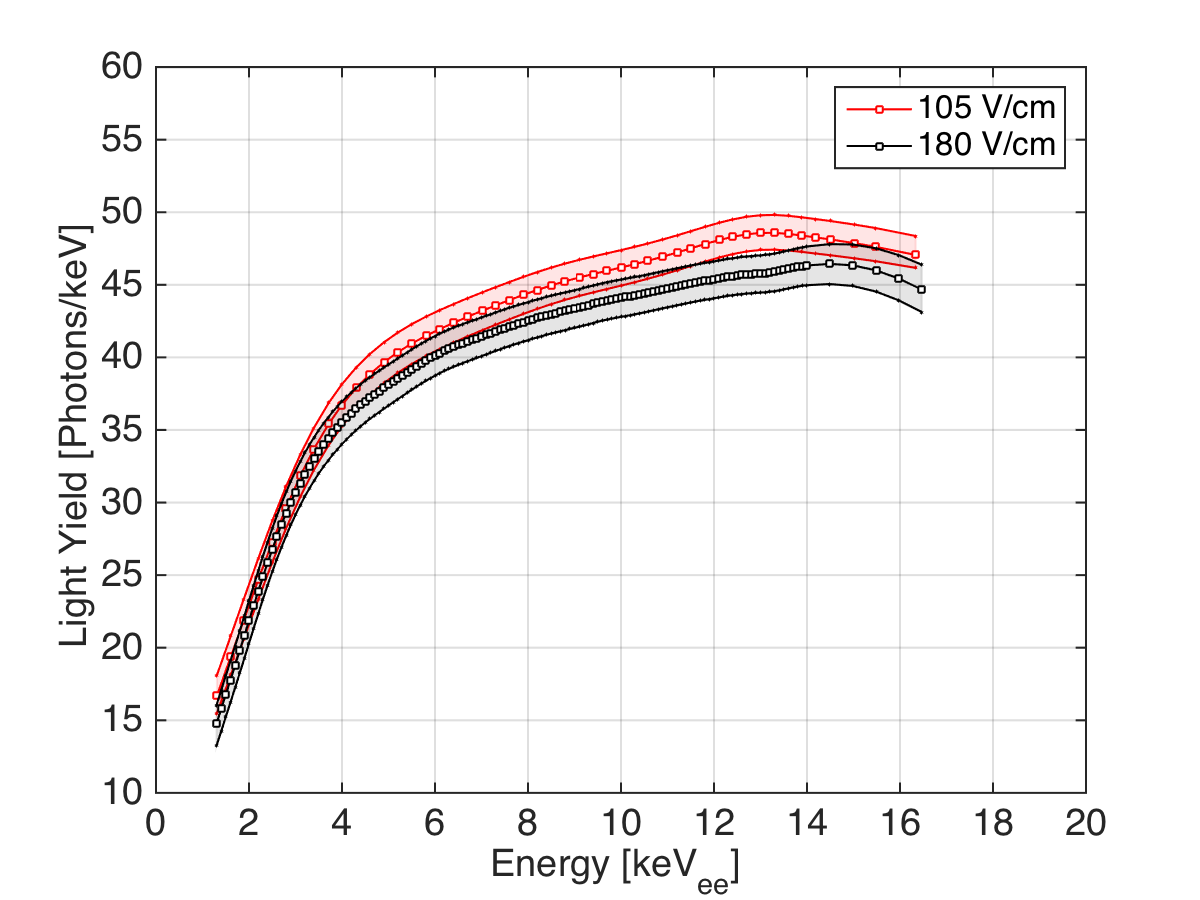
\includegraphics[width=90mm]{fig/ER_LY.png}
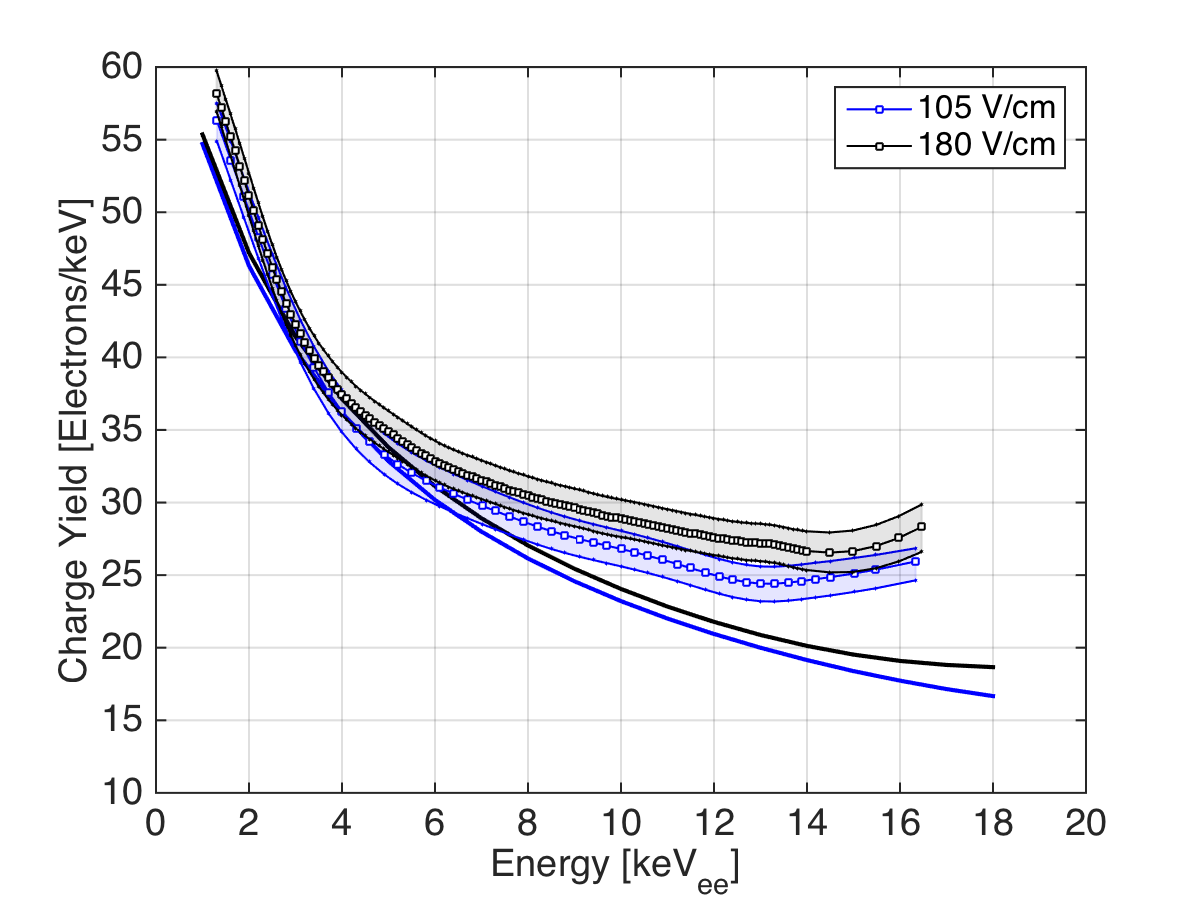
\includegraphics[width=90mm]{fig/ER_QY.png}
\caption{The light yield (upper plot) and charge yield (lower plot) of tritium ER events in LUX at 180~V/cm (black) and 105~V/cm (blue) compared to NEST v0.98 (2013) \cite{NEST_2013}. The NEST curves are solid red and dashed magenta for 105 and 180 V/cm respectively, with triangle markers spaced every one keV. The bands indicate the systematic errors due to $g_1$ and $g_2$, which are fully anti-correlated between the charge yield and light yield across all energy bins. }
\label{fig:ER-LY-QY}
\end{figure}

\begin{table}[h!]
\centering
\begin{tabular}{|c|c|c|c|c|} \hline
Energy 	& 		LY	& 	$\sigma$LY & QY  & $\sigma$QY \\ 
$\rm (keV_{ee}$) & ($\rm n_\gamma$/keV) 	& ($\rm n_\gamma$/keV) & ($\rm n_e$/keV) & ($\rm n_e$/keV) \\ \hline
1.3 	 & 14.6 	 & 3.7 	 & 58.4 	 & 3.7 \\ \hline 
1.5 	 & 17.2 	 & 1.3 	 & 55.8 	 & 1.3 \\ \hline 
2.0 	 & 21.9 	 & 0.4 	 & 51.1 	 & 0.4 \\ \hline 
2.5 	 & 27.3 	 & 0.7 	 & 45.7 	 & 0.7 \\ \hline 
3.0 	 & 31.3 	 & 0.7 	 & 41.7 	 & 0.7 \\ \hline 
3.5 	 & 33.7 	 & 0.8 	 & 39.3 	 & 0.8 \\ \hline 
4.0 	 & 35.6 	 & 0.7 	 & 37.4 	 & 0.7 \\ \hline 
4.5 	 & 37.2 	 & 0.6 	 & 35.7 	 & 0.6 \\ \hline 
5.0 	 & 38.1 	 & 0.6 	 & 34.9 	 & 0.6 \\ \hline 
5.2 	 & 38.8 	 & 0.7 	 & 34.2 	 & 0.7 \\ \hline \hline
5.2$^*$ 	 & 40.9 	 & 1.2 	 & 31.3	 & 2.2 \\ \hline \hline
5.5 	 & 39.3 	 & 0.6 	 & 33.7 	 & 0.6 \\ \hline 
6.0 	 & 40.3 	 & 0.7 	 & 32.7 	 & 0.7 \\ \hline 
6.5 	 & 41.2 	 & 0.6 	 & 31.8 	 & 0.6 \\ \hline 
7.0 	 & 41.8 	 & 0.7 	 & 31.2 	 & 0.7 \\ \hline 
7.5 	 & 42.3 	 & 0.6 	 & 30.7 	 & 0.6 \\ \hline 
8.0 	 & 42.9 	 & 0.5 	 & 30.1 	 & 0.5 \\ \hline 
9.0 	 & 43.7 	 & 0.6 	 & 29.3 	 & 0.6 \\ \hline 
10.0 	 & 44.5 	 & 0.4 	 & 28.5 	 & 0.4 \\ \hline 
11.0 	 & 45.3 	 & 0.8 	 & 27.7 	 & 0.8 \\ \hline 
12.0 	 & 45.8 	 & 0.9 	 & 27.2 	 & 0.9 \\ \hline 
13.0 	 & 46.5 	 & 0.9 	 & 26.5 	 & 0.9 \\ \hline 
14.0 	 & 47.0 	 & 1.0 	 & 26.0 	 & 1.0 \\ \hline 
16.0 	 & 46.3 	 & 1.6 	 & 26.7 	 & 1.6 \\ \hline 
17.0 	 & 45.2 	 & 1.5 	 & 27.8 	 & 1.5 \\ \hline 
\end{tabular}
\caption{Light and charge yield (photons/keV and electrons/keV) measured with tritium decay 180 V/cm. $^*$ 5.2 keV x-ray from $\rm ^{127}Xe$ decay in the WS data.}
\label{table:Yields}
\end{table}

\begin{table}[h!]
\centering
\begin{tabular}{|c|c|c|c|c|} \hline
Energy 	& 		LY	& 	$\sigma$LY & QY  & $\sigma$QY \\ 
$\rm (keV_{ee}$) & ($\rm n_\gamma$/keV) 	& ($\rm n_\gamma$/keV) & ($\rm n_e$/keV) & ($\rm n_e$/keV) \\ \hline
1.3 	 & 18.5 	 & 1.6 	 & 54.5 	 & 1.6 \\ \hline 
2.2 	 & 25.5 	 & 0.7 	 & 47.5 	 & 0.7 \\ \hline 
3.1 	 & 33.3 	 & 1.0 	 & 39.7 	 & 1.0 \\ \hline 
4.0 	 & 37.2 	 & 1.0 	 & 35.8 	 & 1.0 \\ \hline 
4.9 	 & 40.0 	 & 0.7 	 & 33.0 	 & 0.7 \\ \hline 
5.8 	 & 41.3 	 & 0.7 	 & 31.7 	 & 0.7 \\ \hline 
6.7 	 & 43.2 	 & 0.9 	 & 29.8 	 & 0.9 \\ \hline 
7.6 	 & 44.3 	 & 0.6 	 & 28.7 	 & 0.6 \\ \hline 
8.5 	 & 46.5 	 & 1.8 	 & 26.5 	 & 1.8 \\ \hline 
9.4 	 & 46.3 	 & 1.2 	 & 26.7 	 & 1.2 \\ \hline 
10.3 	 & 47.9 	 & 0.6 	 & 25.1 	 & 0.6 \\ \hline 
11.2 	 & 46.7 	 & 0.5 	 & 26.3 	 & 0.5 \\ \hline 
12.1 	 & 48.5 	 & 0.8 	 & 24.5 	 & 0.8 \\ \hline 
13.0 	 & 49.2 	 & 0.7 	 & 23.8 	 & 0.7 \\ \hline 
13.9 	 & 50.6 	 & 1.9 	 & 22.4 	 & 1.9 \\ \hline 
15.0 	 & 51.0 	 & 3.5 	 & 22.8 	 & 2.7 \\ \hline 
16.3 	 & 48.8 	 & 2.3 	 & 24.1 	 & 2.3 \\ \hline 
\end{tabular}
\caption{Light and charge yield (photons/keV and electrons/keV) measured with tritium decay at 105 V/cm }
\label{table:Yields_100}
\end{table}


The light yield measurements are compared to similar measurements by other authors in Fig. \ref{fig:Re_LY}. To remove detector effects from this comparison, the light yield is normalized to that of the 32.1~keV electron capture decay of $\rm ^{83m} Kr$ at zero electric field. For LUX this light yield is measured to be $ 63.3 \pm 3$ photons/keV. Although the error bars on the comparison data are large, the findings are consistent with the expectation that the tritium light yields at 105 and 180~V/cm lie between those at zero field and 450~V/cm from \cite{Aprile_LY} and \cite{Baudis}. It is worth noting that Refs. \cite{Aprile_LY} and \cite{Baudis} use Compton scatters as the source of ER events, while in tritium data the ER source is a beta decay. At low energy beta decays and Compton scatters will leave similar track lengths and produce similar event characteristics. \fixit{We have also included the 5.2 keV x-ray from $\rm ^{127}Xe$ in the WS data (180 V/cm), which is in good agreement with the tritium result}. The comparison of Fig. \ref{fig:Re_LY} supports this expectation, albeit with the large experimental uncertainties.

\begin{figure}[h!]
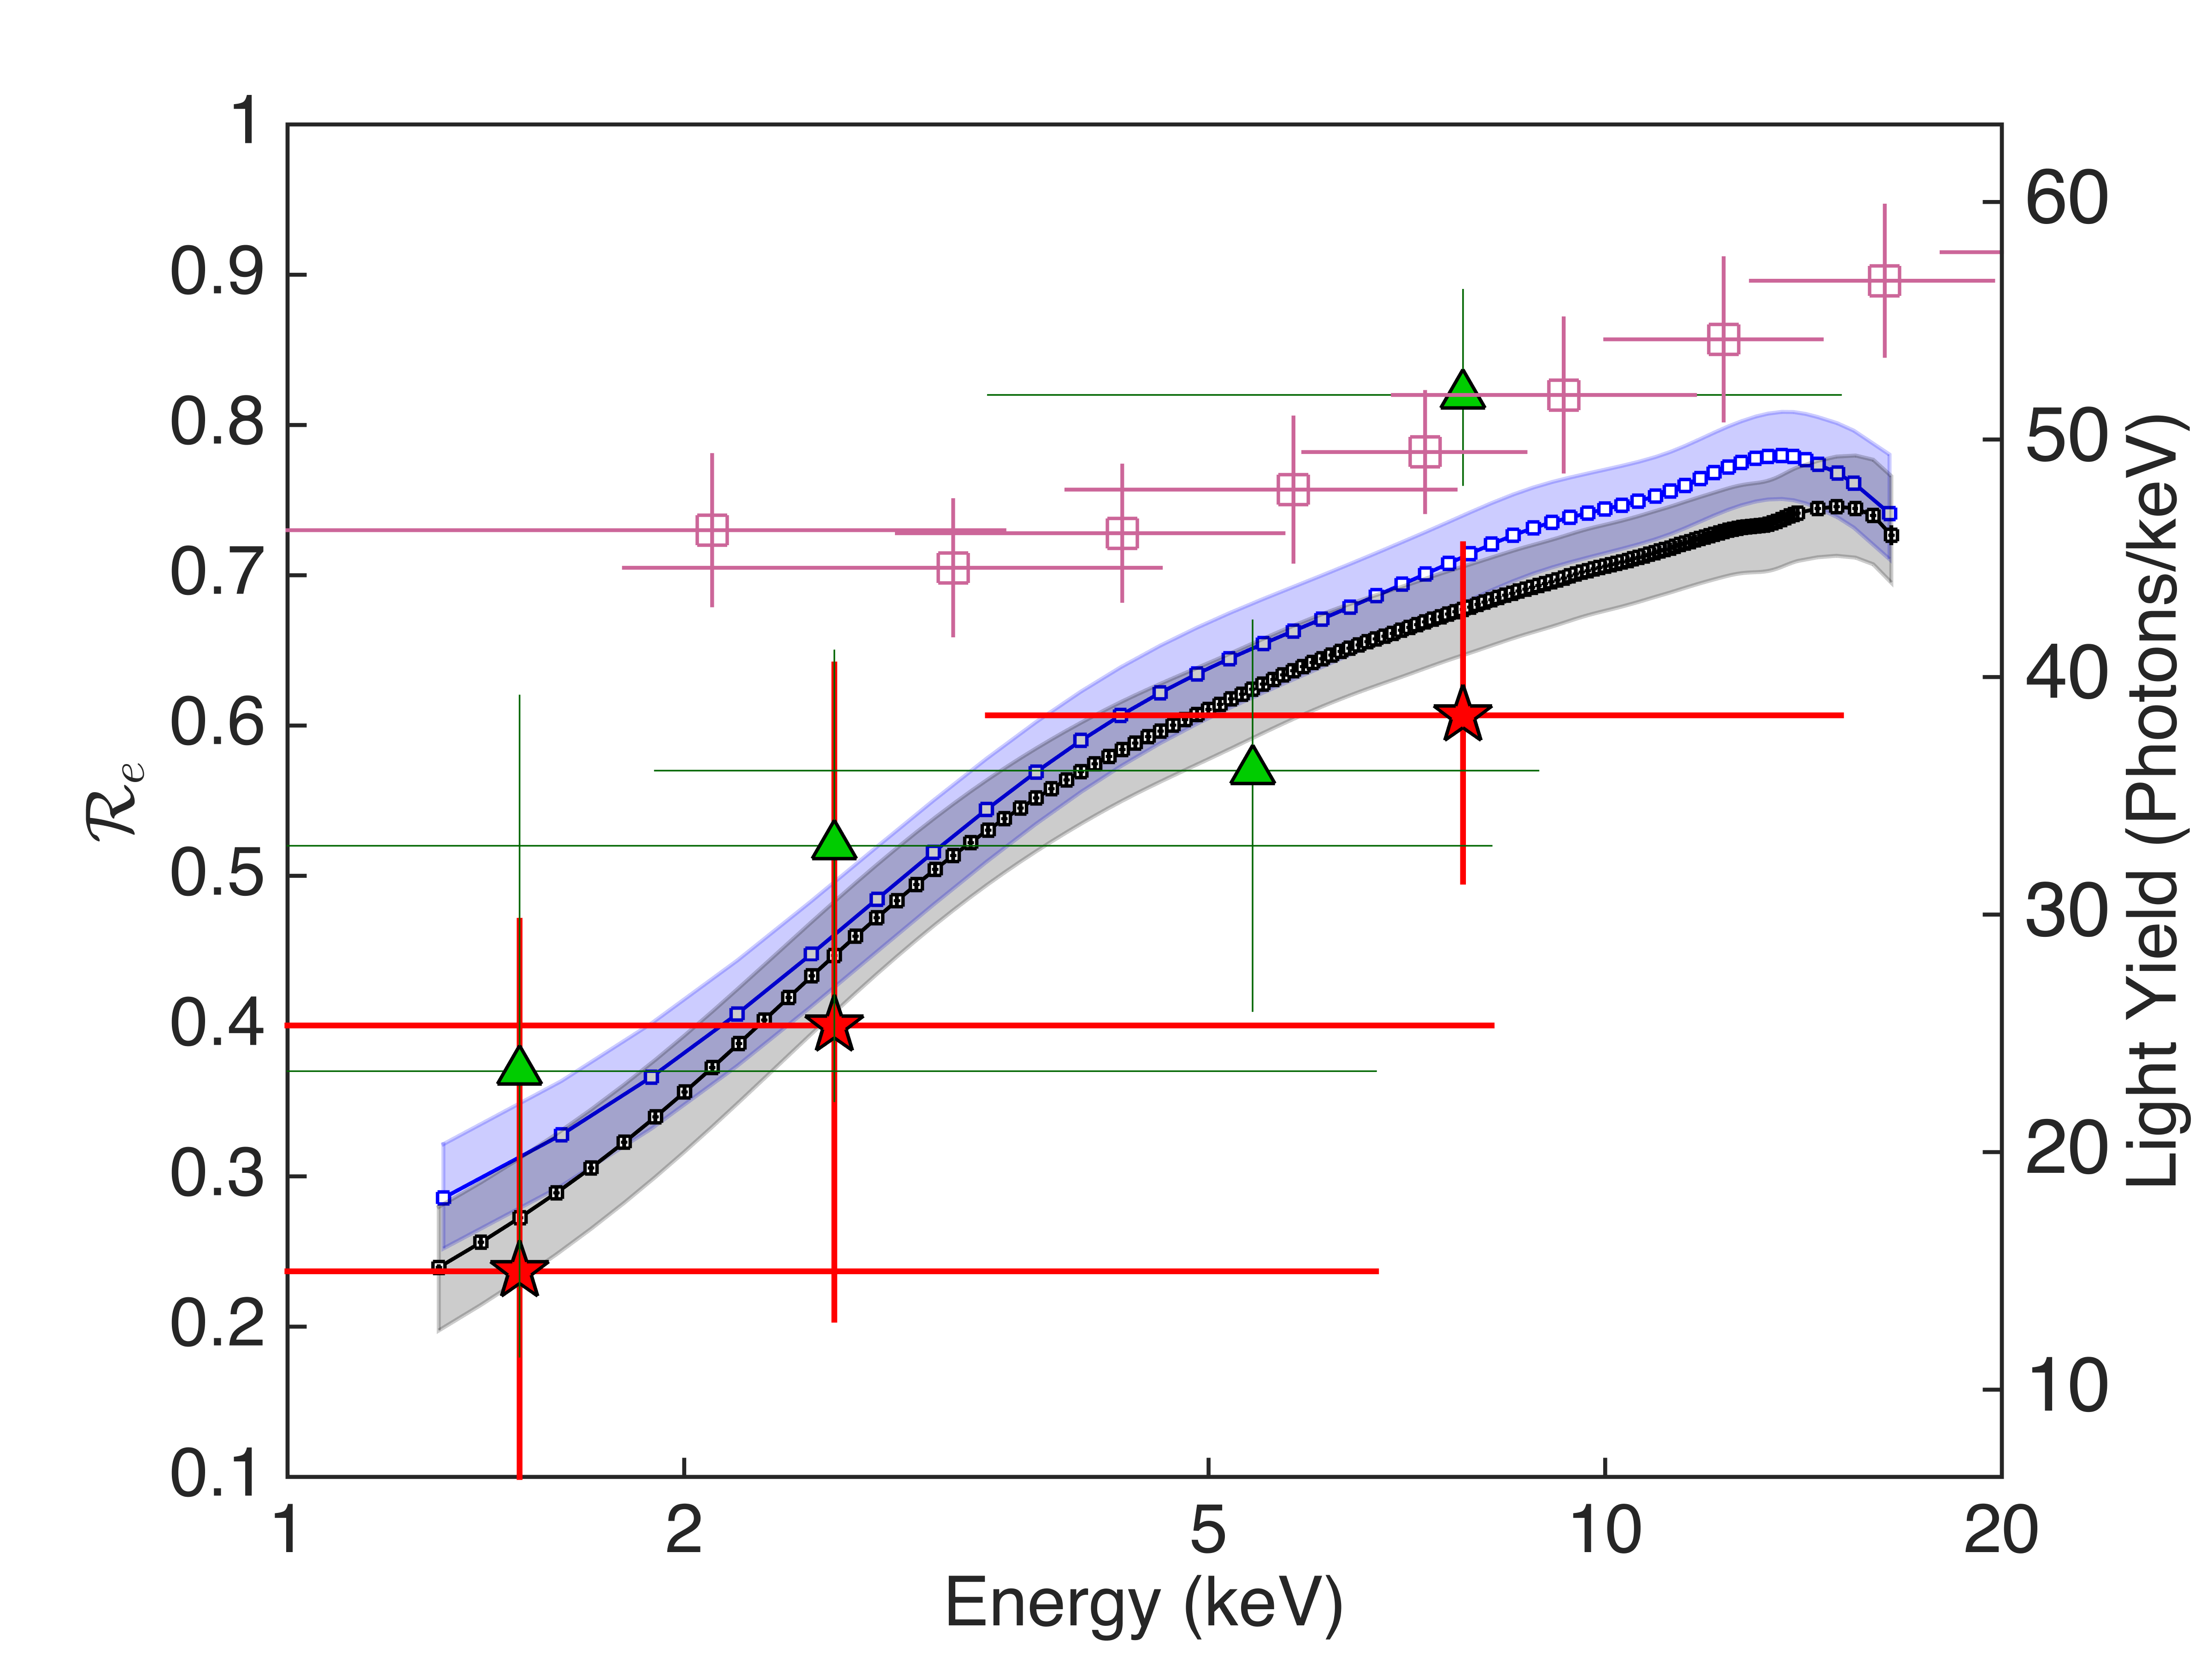
\includegraphics[width=88mm]{fig/Re_LY_log.png}
\caption{Light yield measurement from LUX tritium data compared with results from other authors. Left vertical scale: light yield relative to that of the 32.1~keV decay of $\rm ^{83m}Kr $ at zero field. Right vertical scale: absolute light yield measurements. Shaded blue curve is tritium at 105~V/cm, shaded black curve is tritium at 180~V/cm. \fixit{Green square is the 5.2 keV x-ray from $\rm ^{127}Xe$ in the WS data at 180 V/cm}. Magenta squares represent zero field measurements from \cite{Aprile_LY}, cyan triangles and red circles represent zero field and 450~V/cm from \cite{Baudis}. All non-tritium data is from Compton scatters. }
\label{fig:Re_LY}
\end{figure}


As shown in Fig. \ref{fig:ER-LY-QY}, we find that the light yield increases rapidly from 1 to 6~keV, and then becomes mostly energy independent over the remainder of the tritium spectrum. The charge yield exhibits the reverse behavior, lending support to the combined energy model. 

\begin{figure}[h!]
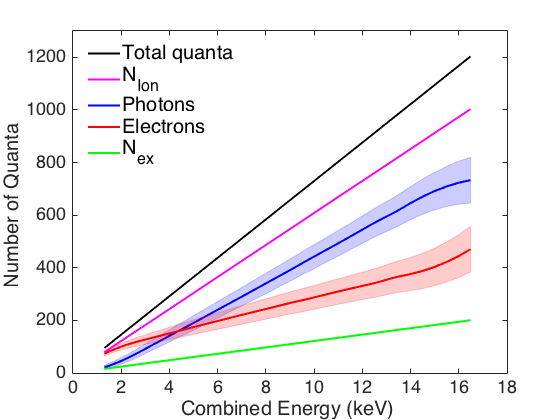
\includegraphics[width=90mm]{fig/quanta-vs-energy.png}
\caption{Top: The mean number of electrons (red) and scintillation photons (blue) produced in LUX at 180~V/cm as a function of energy. The bands indicate the correlated systematic errors on $g_1$ and $g_2$. Also shown are the total number of quanta, primary ions, and primary excitons, assuming an exciton to ion ratio of 0.2. }
\label{fig:quanta-vs-energy}
\end{figure}

We understand this behavior as due to the effects of recombination, the process by which newly liberated ionization electrons are captured by Xe$^+$ ions, creating additional Xe$^*$ excitons, and ultimately scintillation photons. We model recombination as follows. Starting with a $W$-value of 13.7~eV, we assume that $\alpha$, the initial ratio of excitons-to-ions prior to recombination, is 0.2 independent of energy and electric field~\cite{Doke_alpha}. Then the initial number of ions prior to recombination ($N_{ion}$, equivalent to the initial number of electrons), and the initial number of excitons prior to recombination ($N_{ex}$), and their sum (the total number of quanta), all increase linearly with energy as shown by the solid lines in Fig. \ref{fig:quanta-vs-energy}. Also shown in Fig. \ref{fig:quanta-vs-energy} are the total observed number of electrons and scintillation photons after recombination measured with the LUX tritium data at 180~V/cm as a function of energy. The sum of the observed electrons and photons should also increase linearly with energy, a hypothesis which is tested and confirmed by the tritium spectrum comparison of Fig. \ref{fig:tritium-spectrum}.

We see that at very low energy, below 3~keV, the number of electrons and photons is similar to $N_{ion}$ and $N_{ex}$, respectively, while above 4~keV the number of electrons drops below the number of photons, consistent with a large recombination effect at these energies and this electric field. The recombination fraction, calculated according to

\begin{equation}
r = \frac{(n_{\gamma}/n_e) - \alpha}{(n_{\gamma}/n_e) + 1},
\end{equation}

\noindent
is shown explicitly in Fig. \ref{fig:recombination}, measured with both the 180~V/cm and 105~V/cm tritium data. We find only a small difference in the recombination between these two field values in this energy range. It is worth noting that recombination is small at the very lowest energies where the dark matter search is performed, rapidly approaching zero as the energy drops below 4~keV. As noted before, this behavior is of significant importance for the efficacy of recoil discrimination in LXe~\cite{xed-discrimination}. Other authors have used $\alpha$ values between 0.06 and 0.2~\cite{kaixuan}. Changing the value of $\alpha$ modestly affects the absolute magnitude of the resulting recombination fraction but has only a small affect on the shape as a function of energy. 

\begin{figure}[h!]
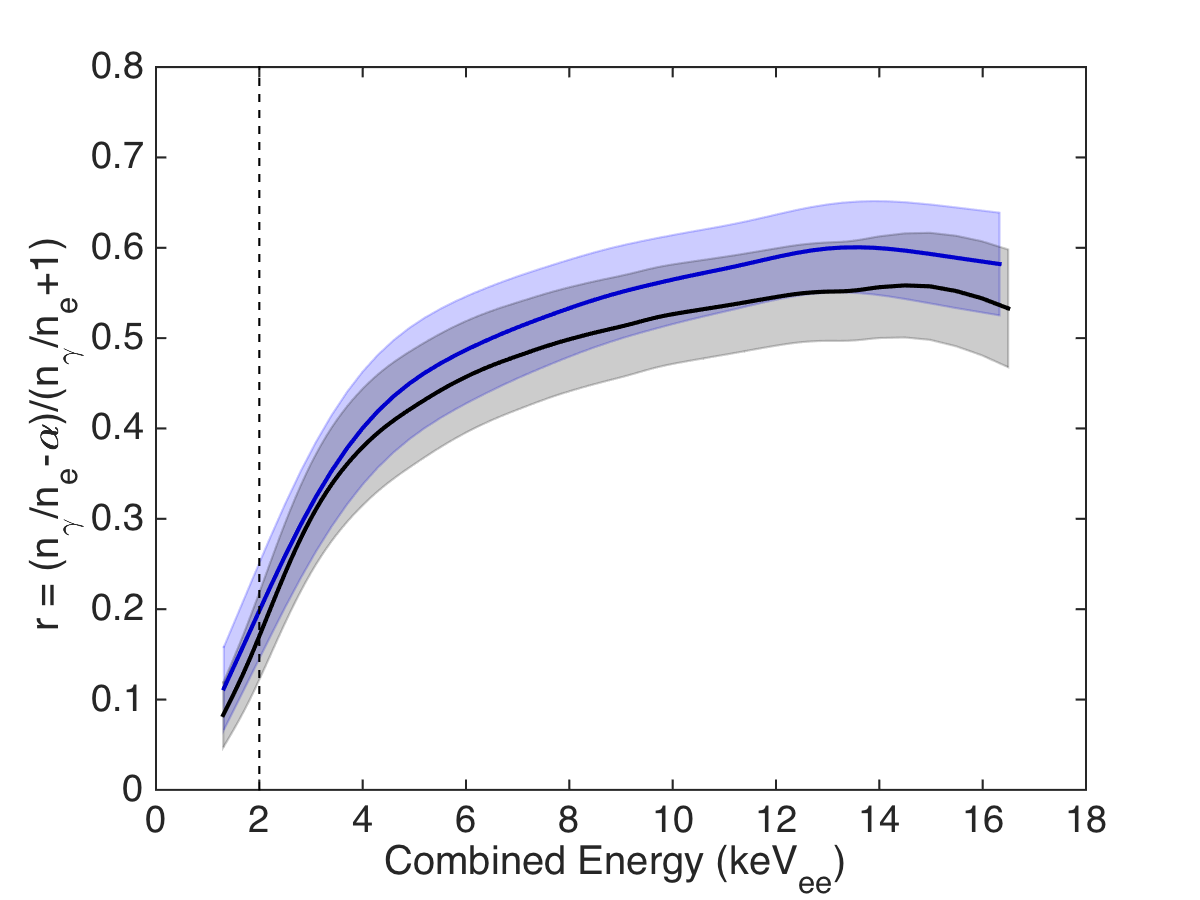
\includegraphics[width=90mm]{fig/recombination.png}
\caption{Recombination fraction of ER events at 180~V/cm (black) and 105~V/cm (blue), assuming an exciton-to-ion ratio of 0.2.}
\label{fig:recombination}
\end{figure}

\begin{figure}[h!]
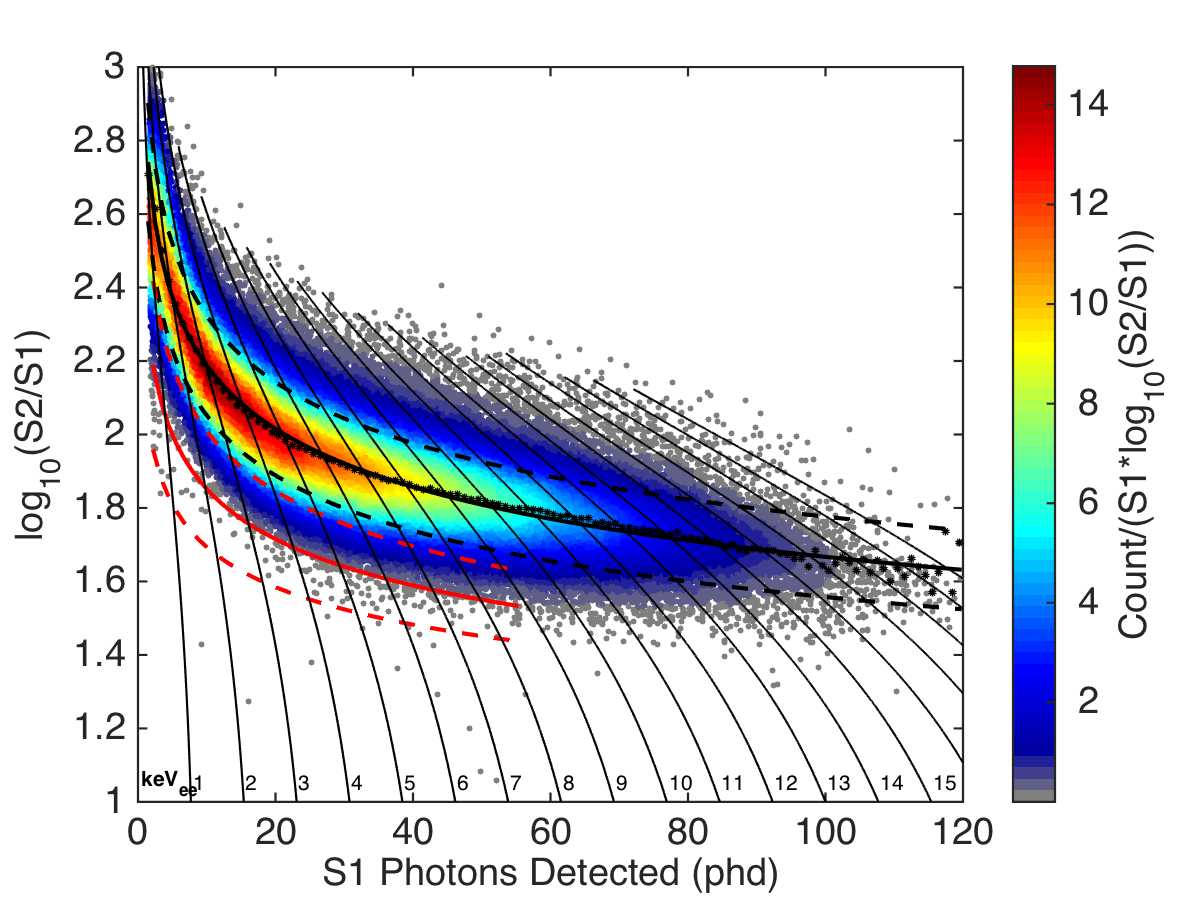
\includegraphics[width=90mm]{fig/CH3T_ER_Band.png}
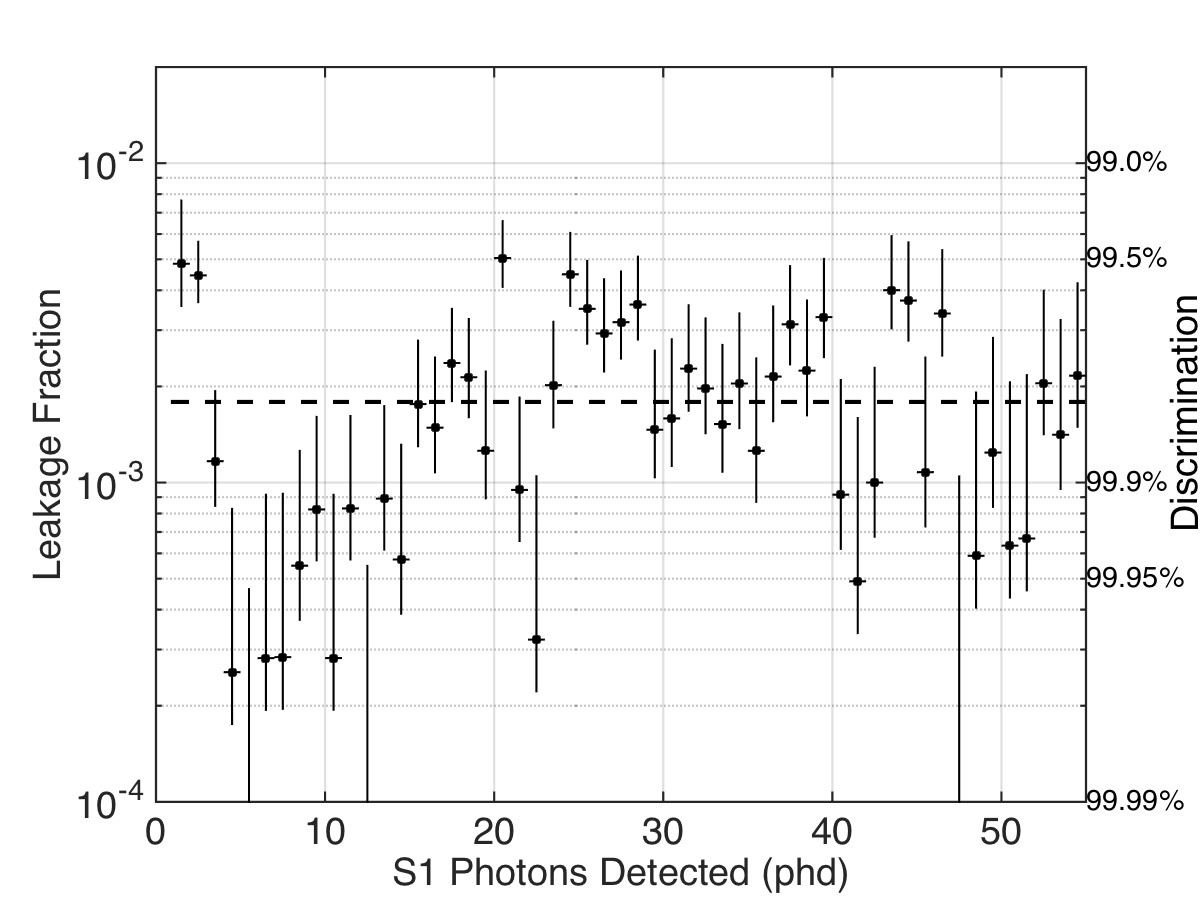
\includegraphics[width=85mm]{fig/CH3T_Leakage_Run03.png}
\caption{Top: The electron recoil band of LUX illuminated by 170,000 tritium events at the nominal LUX electric field of 180~V/cm.  The recoil discriminant variable, log(S2/S1), is shown vs. S1 between 1 and 120 phd in S1 (with contours of constant energy $1-20 \, keV_{ee}$). Also indicated in black are the mean and the 10\% and 90\% contours of the ER population. The solid red line represents the mean NR band determined with DD neutron generator data. The dashed red indicates the 10\% and 90\% contours of the NR band. Bottom: Observed LUX recoil discrimination vs. S1, defined as the fraction of events below the NR mean. Y-axis labels: left -  leakage fraction ($f$); right - discrimination ($1-f$).}
\label{fig:ER_band}
\end{figure}

The LUX ER band is shown as log$_{10}$(S2/S1) vs S1 in Fig. \ref{fig:ER_band}(top).  Also shown is the NR band measured with neutron generator data\cite{DD-paper, lux-reanalysis}. The ER band has a characteristic rise at decreasing values of S1 which reflects the rapidly changing charge and light yields below $\sim$6~keV. The leakage fraction ($f$), defined as the fraction of ER events observed below the mean of the NR band, is shown in Fig. \ref{fig:ER_band}(bottom) as a function of S1. The recoil discrimination efficiency ($1-f$) has an average value of 99.81 $\pm$ 0.02\% for events with S1 between 1 and 50 phd.


\onecolumngrid
\break
\begin{sidewaysfigure}[p!]
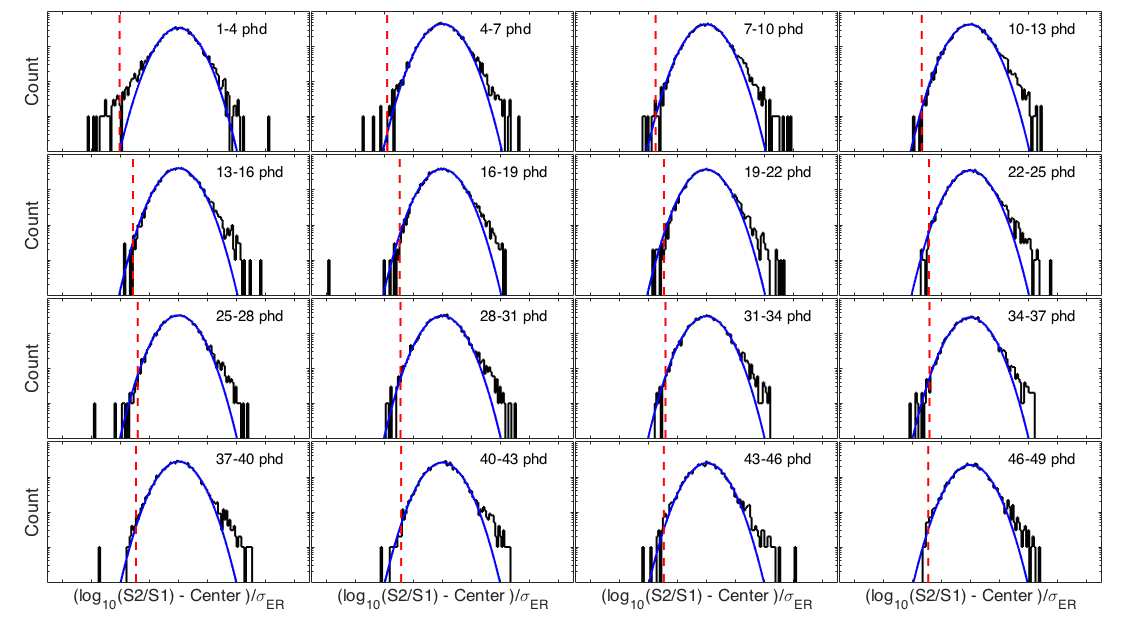
\includegraphics[width=220mm]{fig/Gaussianity/GaussER_all.png}
\caption{Electron recoil population from tritium events about the centroid of the mean in 3 phd bins over over the WIMP region of interest (1 - 49 phd). We fit each bin to a Gaussian, and subtract the centroid of the Gaussian. The x-axis is measured in units of the fitted Gaussian width. The red dashed line represents the mean of the NR band in each bin. We observe non Gaussian behavior below three sigma of the ER band and two sigma above.  }
\label{fig:ER-Gauss}
\end{sidewaysfigure}
\twocolumngrid


In Fig. \ref{fig:ER-Gauss} we histogram $ log_{10}(S2/S1)$ in bins of S1 with a bin-width of 3 phd. In each bin we show a Gaussian fit to the data after subtracting the centroid and dividing by the Gaussian width. We find that the Gaussian fits describe the data well out to about $2\sigma$ on the upper side and $3\sigma$ on the lower side, beyond which non-Gaussian tails are visible.  \fixit{The tritium data sets used here contain 27.5 live hours of data. Within the time window of data acquisitions and in a range of 1-18 $\rm keV_{ee}$ less than 15 ER events from backgrounds are expected, these would not contribute significantly to non-gaussian tails. Nuclear recoils from alpha decays on the walls with improperly reconstructed position would show up as extreme outliers well below four sigma of the ER band,  however the rate of these is 0.5 per day. Another background to consider is accidental coincidence tritium events where an S1 originating from below the cathode, thus not having an S2, is paired with a low energy S2 in the fiducial for which the S1 signal fell below threshold. The expected number of accidental coincidence events in the tritium data sets is 2.5. With only 2.5 accidental-coincidental tritium events and 0.5 alpha events from the wall expected to be present out of 170,000 events total the small non-Gaussian tails appear to be a genuine feature of ER events in LUX}. \fixit{However, it is uncertain whether the non-Gaussian tails originate as a detector effect or due to the fundamental physics of liquid xenon.} 
 

In general the width of the ER band should be comprised of three components: the uncertainties on  $n_{\gamma}$ and $n_e$  due to detector resolution ($ \sigma(n_{\gamma})$ and $ \sigma(n_e)$), and true event-to-event variations in recombination ($ \sigma(R)$). $ \sigma(n_{\gamma})$ and $ \sigma(n_e)$ are responsible for fluctuations in the vertical  and horizontal directions in Fig. \ref{fig:tritium-scatter},  while 
$ \sigma(R)$ causes fluctuations along the diagonal lines of constant energy. $ \sigma(n_{\gamma})$ and $ \sigma(n_e)$ can be measured as a function of energy and are shown in Fig. \ref{fig:recomb-flucs} for LUX tritium data at 180~V/cm\cite{Dobi_Thesis}. Also shown in Fig. \ref{fig:recomb-flucs} is the extracted value of $ \sigma(R)$ as a function of energy after controlling for $ \sigma(n_{\gamma})$ and $ \sigma(n_e)$ by a method described in Ref. \cite{Dobi_Thesis}. 

\begin{figure}[h!]
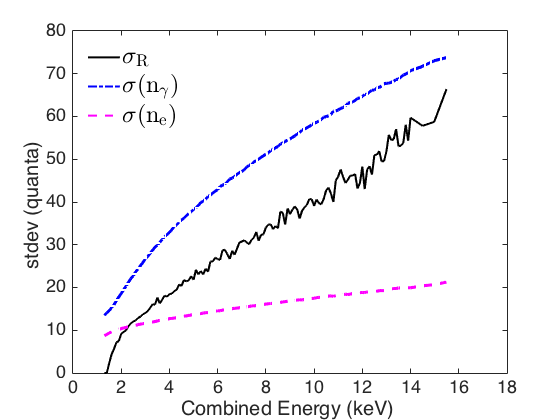
\includegraphics[width=90mm]{fig/recomb_flucs.png}
\caption{Black: recombination fluctuations in LXe measured with LUX tritium data at 180~V/cm. Dot-dash blue: Detector resolution for counting photons. Dashed magenta: Detector resolution for counting electrons.}
\label{fig:recomb-flucs}
\end{figure}

We find that at 180~V/cm in LUX, $ \sigma(n_{\gamma})$ is the most important contributor to the ER band width over the entire tritium energy spectrum. Between 2 and 6~keV, where the WIMP search is most sensitive, $ \sigma(n_e)$ and $ \sigma(R)$ are of comparable magnitude and secondary importance. We note that an ideal detector would be limited by only $ \sigma(R)$.


%Having measured the light and charge yield in-situ we have an understanding of the mean of the electron recoil population for the LUX the WIMP search. To complete the picture we need to understand the variance that lead to the width of the electron recoil band. This is comprise of detector resolution, which is measurable and specific to each detector, and recombination fluctuations. At a given energy the event-to-event standard deviation for the number of recombined ions $ \sigma(R)$ is shown in Fig. \ref{fig:recomb-flucs}, extracted using a method outlined in \cite{Dobi_Thesis}. $ \sigma(R)$ is a physical property of xenon and produces and irreducible width to the electron recoil band, even with infinite detector resolution. Currently no models exist to predict recombination fluctuations ($ \sigma(R)$), thus it is important to measure it in-situ. For the LUX detector conditions we find a linear growth in recombination fluctuations as a function of the number of ions $ \sigma(R) = (0.062 \pm 0.005)\cdot N_{ions}$, consistent with the measurement in \cite{Dobi_Thesis}.



%% ER band Gaussianity section. If we want this


%%%%%%%%%%%%%%%%%%%%%%%%%%%%%%%%%%%%%%%%%%%%%%%%%%%%%%%%%%

